% !TeX spellcheck = en_US
\chapter{Experiments on Real Hardware}\label{ch:real}%

This chapter describes the physical system and reports the hardware experiments. Section~\ref{sec:real-setup} covers the robot, the camera and its calibration, the controller, and the measurement of the nut angle. Section~\ref{sec:real-transfer} describes the zero-shot transfer protocol. Section~\ref{sec:real-results} reports the closed-loop results of the distilled student on the training nut sizes, Section~\ref{sec:real-geometry} on unseen nut geometries, and Section~\ref{sec:real-stress} under long-horizon stress.

\section{Hardware Setup}\label{sec:real-setup}

The physical platform comprises the same FR3 arm and Inspire RH56DFX hand as the simulation, mounted at tabletop height in front of a bench that carries the bolt on its pedestal (Figure~\ref{fig:real-setup}). The hand is attached through a 10\,mm adapter flange whose transform was measured and reproduced in the simulated asset; the asset itself was regenerated from the manufacturer's URDF so that joint limits, link inertias, and the mechanical coupling of the finger joints match the physical hand. An Intel RealSense D415 mounted on a fixed stand provides the RGB-D observation at $640\times480$, which is center-cropped and downscaled to the $320\times180$ policy input as in simulation. Its pose relative to the robot base was measured by an eye-to-hand calibration with a translation fit RMSE of 27\,mm and a rotation fit RMSE of $3.5\degree$ over the calibration poses; the calibrated optical pose and the intrinsics are the ones used to render the simulated camera and to back-project the point cloud, so that the student sees the same geometry in both domains.
% TODO(unsure): the calibration artifact is labeled "measured", not "deployment validated"; confirm whether a refined calibration was used for the reported hardware trials.

Robot commands use the same Cartesian impedance law as in simulation. The deployment controller is the libfranka Cartesian-impedance example controller, which applies $\vec{\tau}=\mat{J}^{\mathrm{T}}(\mat{K}\vec{e}-\mat{D}\dot{\vec{x}})$ with a quaternion-vector orientation error, a nullspace term through a damped Jacobian pseudoinverse, and the robot's own Coriolis and gravity compensation, at the 1\,kHz rate of the Franka control interface, while the student commands targets at 15\,Hz. The hand is position-controlled through its serial interface. The gains of the deployment controller and the mapping of the student's bounded action to the controller target are \tbd.
% TODO(results): document the physical controller gains, the target low-pass settings, and the hand command rate used in the hardware trials (libfranka tooling on the franka-chi branch).

\paragraph{Controller families.}
The simulated Factory controller and the physical libfranka-style controller share the task-space law of \eqref{eq:osc} but differ in the nullspace projector. The Factory controller uses the undamped, dynamically consistent torque projector built from the joint-space inertia, whereas the libfranka example uses a damped kinematic projector built from a regularized pseudoinverse of the Jacobian transpose with regularization 0.2, and it adds the robot's Coriolis term, which the simulator supplies in the matching simulated backend. Both backends are implemented in the simulation with selectable gains, so that a teacher can be trained under either. The reported teachers use the Factory gains, and the physical controller is tuned toward them rather than the other way around, so that the student's commands meet the stiffness under which the teacher acquired its contact behavior.

\paragraph{Trajectory export.}
For open-loop validation of the action path, every simulated demonstration can be exported as a command-only deployment artifact. The simulator recording is authoritative for the geometric joint path; because some scripted phases change the joint position kinematically while writing zero articulation velocity, the export does not use recorded velocities but fits one twice continuously differentiable quintic curve through the recorded positions and derives position, velocity, and acceleration from it, with deployment limits on joint positions and velocities applied explicitly. Rows with a valid controller command also retain the recorded reverse-engineered 17-D impedance command, so that a joint-space replay is possible on controllers that do not expose a Cartesian interface. On the FR3 the Cartesian targets are executed directly through the libfranka-style controller, which keeps open-loop playback and student execution on the same path.

The nut angle that the metrics of Section~\ref{sec:metrics} require is read from an angular scale printed on a sheet under the bolt pedestal (Figure~\ref{fig:real-phases}); the unwrapped angle is recorded at the end of every goal-reaching phase. The test-object family, shown in Figure~\ref{fig:real-setup} on the right, consists of M24, M30, and M36 nuts in four profiles each, hexagonal, octagonal, rectangular, and round, with matching bolts and holders. Teacher and student training use the hexagonal profiles only; the other three profiles are held out for the generalization study of Section~\ref{sec:real-geometry}.

\begin{figure}[htb]%
    \centering%
    \begin{subfigure}[b]{0.49\textwidth}
        \centering
        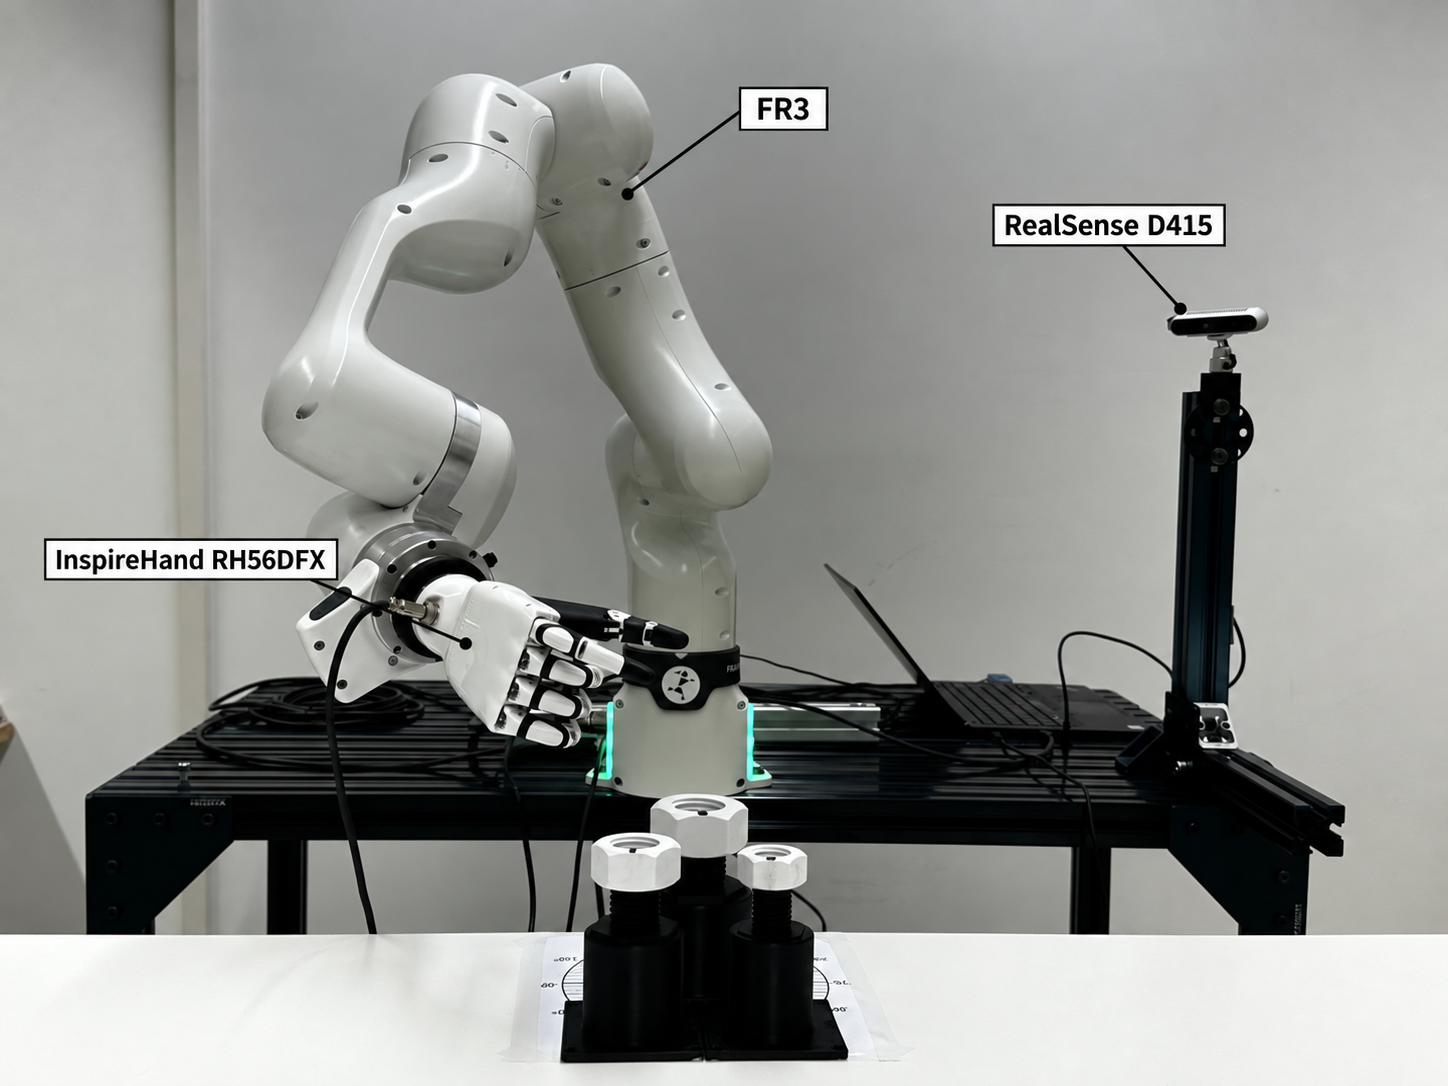
\includegraphics[width=\textwidth]{figures/hardware_setup_annotated.png}
        \caption{Physical workcell.}
    \end{subfigure}\hfill
    \begin{subfigure}[b]{0.49\textwidth}
        \centering
        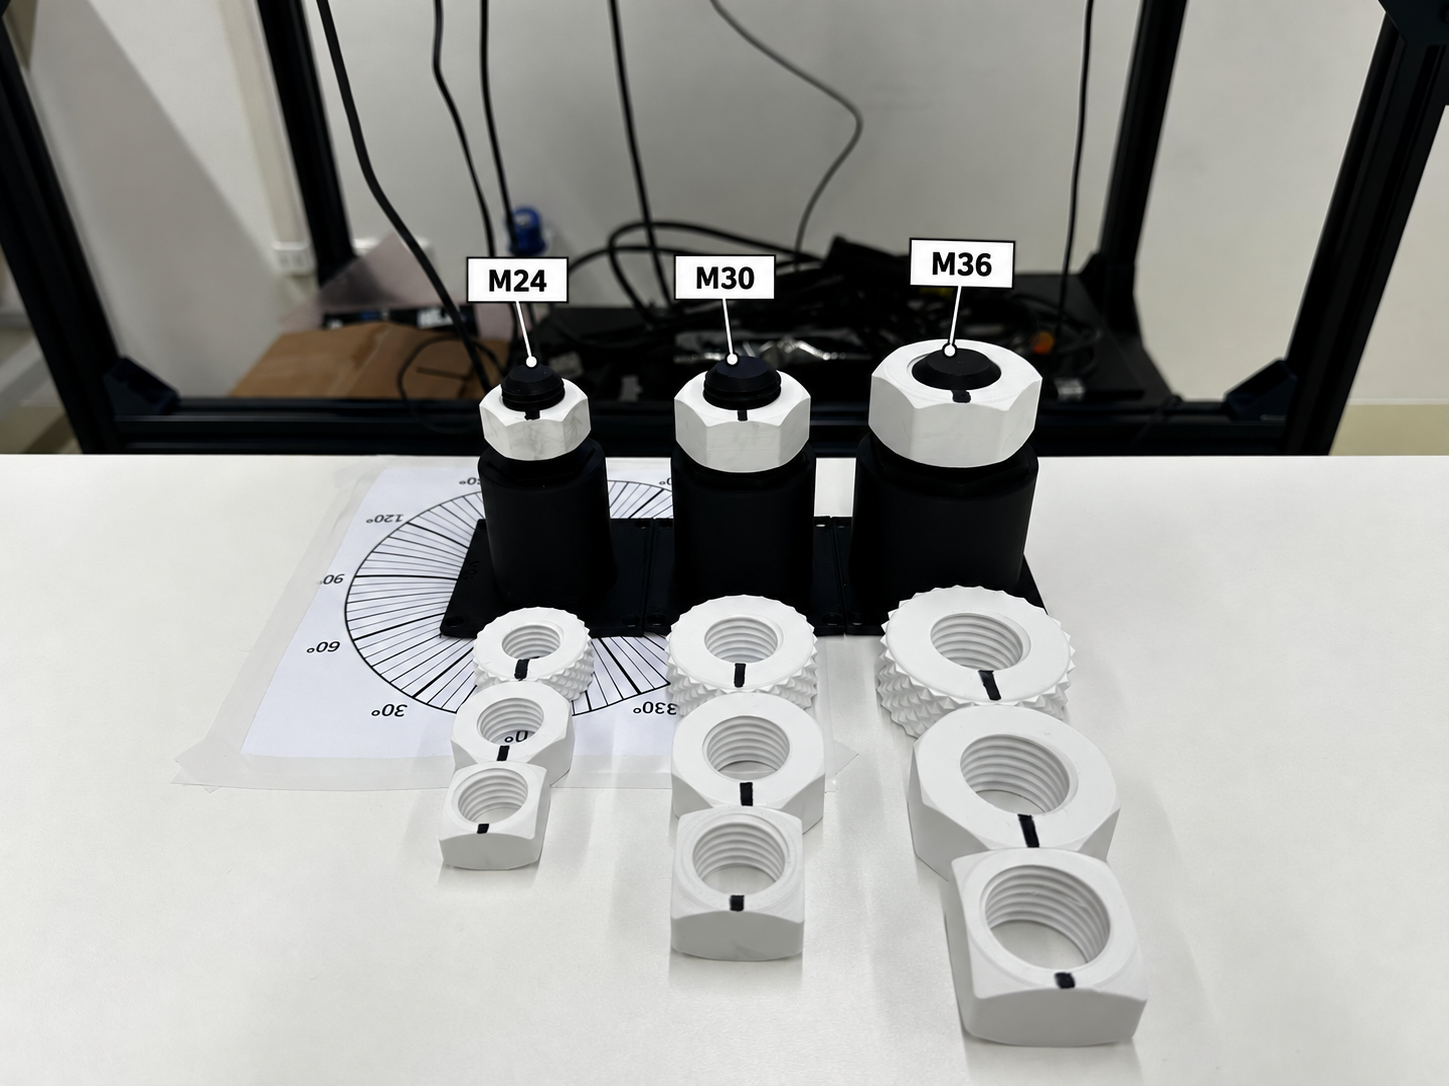
\includegraphics[width=\textwidth]{figures/NutBoltHolderFamilyOnly2_annotated.png}
        \caption{Test-object family.}
    \end{subfigure}
    \caption{Hardware setup. Left: the FR3 arm with the Inspire RH56DFX hand, the bolts on their holders in front of the robot, and the fixed RealSense D415 on its stand. Right: M24, M30, and M36 bolts with the hexagonal, octagonal, rectangular, and round nuts of each size; only the hexagonal nuts are used for training.}%
    \label{fig:real-setup}%
\end{figure}%

\begin{figure}[htb]%
    \centering%
    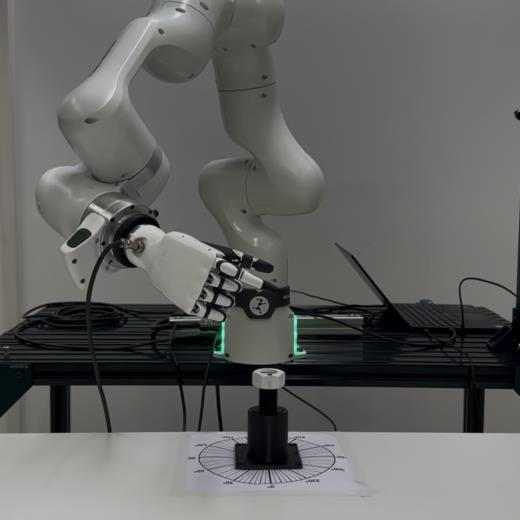
\includegraphics[width=0.19\textwidth]{figures/photos/real_approach.png}\hfill
    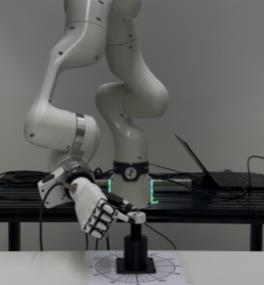
\includegraphics[width=0.19\textwidth]{figures/photos/real_grasp.png}\hfill
    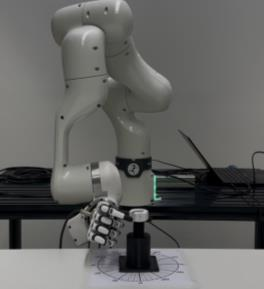
\includegraphics[width=0.19\textwidth]{figures/photos/real_rotate.png}\hfill
    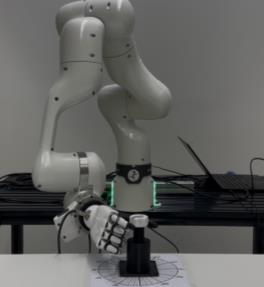
\includegraphics[width=0.19\textwidth]{figures/photos/real_goal.png}\hfill
    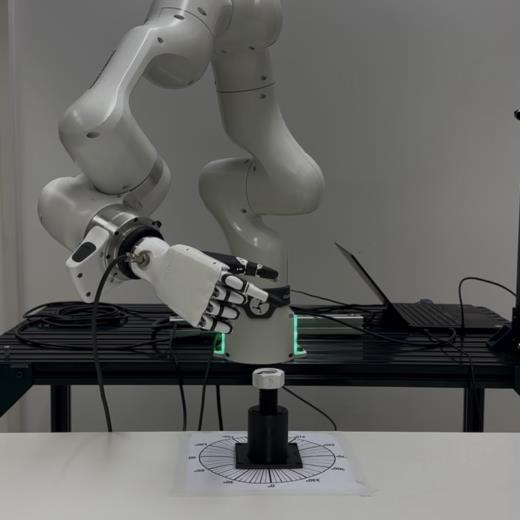
\includegraphics[width=0.19\textwidth]{figures/photos/real_release.png}\\[1mm]
    \hspace*{0.2\textwidth}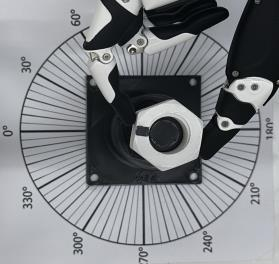
\includegraphics[width=0.19\textwidth]{figures/photos/dial_grasp.png}\hfill
    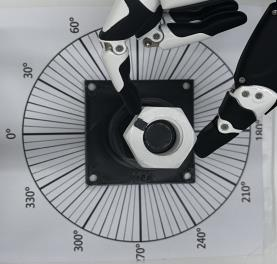
\includegraphics[width=0.19\textwidth]{figures/photos/dial_rotate.png}\hfill
    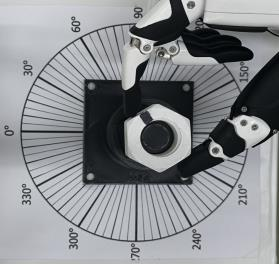
\includegraphics[width=0.19\textwidth]{figures/photos/dial_goal.png}\hspace*{0.2\textwidth}
    \caption{One threading cycle on the physical robot. Top, from left to right: approach, grasp, rotation, goal reaching, and release with return to the reset pose. Bottom: top-down views of the angular scale under the bolt during grasp, rotation, and goal reaching; the scale is read at the end of every goal-reaching phase to compute the cyclic and ten-cycle tracking errors.}%
    \label{fig:real-phases}%
\end{figure}%
% TODO(figure): these photos were taken during the earlier hardware trials; retake them with the zero-shot student, or confirm that they are suitable as an illustration of the phases.

\begin{figure}[htb]%
    \centering%
    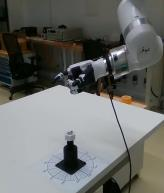
\includegraphics[height=0.3\textwidth]{figures/photos/real_rgb.png}\hspace{6mm}%
    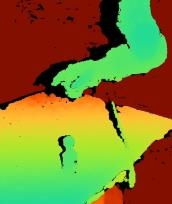
\includegraphics[height=0.3\textwidth]{figures/photos/real_depth.png}
    \caption{Student observation on the physical system: the RGB image (left) and the metric depth image (right) of the RealSense D415 after center-cropping and downscaling to $320\times180$. The depth image is back-projected through the calibrated intrinsics into the point cloud that the student encodes.}%
    \label{fig:real-rgbd}%
\end{figure}%

\section{Zero-Shot Transfer Protocol}\label{sec:real-transfer}

The student of the full method is trained for 300 epochs on the simulated dataset $\Dset=\Dsim$ of Section~\ref{sec:dataset} with eight-step chunks and deployed on the physical robot without any real-world training data, with a prediction horizon of eight and sixteen ODE integration steps. The transfer rests on the four properties of Section~\ref{sec:sim2real}: the calibrated camera of Section~\ref{sec:real-setup} is the one that rendered the demonstrations, the point-cloud crop box removes the physical background before encoding, the demonstrations were rendered under lighting, texture, and background randomization, and the Cartesian targets are executed by the impedance controller described above. The student receives the progress scalar from the elapsed trial time and the process phase from the physical events of the cycle, as in simulation (Section~\ref{sec:student}). Teacher and student training use the hexagonal nuts only.
% TODO(results): document the deployment settings of the zero-shot trials (checkpoint, depth preprocessing on the physical D415, phase-signal source on hardware).

\section{Results on Training Nut Sizes}\label{sec:real-results}

Table~\ref{tab:ablation-real} is the hardware counterpart of the simulation ablation on the M24 hexagonal nut and answers Q4. Three of the five students are taken to hardware: the full method (e), the single-cycle student (a), and the ResNet student (b), which tests whether the image-space representation transfers as well as the point cloud. The two regression heads (c) and (d) are evaluated in simulation only. The hardware results are \tbd.
% TODO(results): run ten zero-shot M24 trials each for (e), (a), and (b) once the simulated-only students are retrained and the randomization ranges are fitted to the physical sensor (Section 3.4.4). For reference: the earlier zero-shot hardware run of the simulated-only student completed 2.1+-1.4 cycles with a cyclic error of -10.05+-4.08 deg; the earlier full-method hardware numbers came from a student trained with real-world replay data and cannot be reused.

\begin{table}[htb]%
    \centering%
    \caption{Real-world zero-shot ablations on the M24 hexagonal nut over ten trials, with the same conventions as Table~\ref{tab:ablation-sim}. Ablations (c) and (d) are evaluated in simulation only.}%
    \label{tab:ablation-real}%
    \small
    \begin{tabular}{lccc}
        \toprule
        Ablation & Completed cycles $\uparrow$ & Cyclic error $\rightarrow0$ & Ten-cycle error $\rightarrow0$ \\
        \midrule
        (a) single-cycle student & \tbd & \tbd & \tbd \\
        (b) ResNet encoder & \tbd & \tbd & \tbd \\
        (e) full method & \tbd & \tbd & \tbd \\
        \bottomrule
    \end{tabular}
\end{table}%

\section{Generalization across Nut Sizes and Geometries}\label{sec:real-geometry}

Table~\ref{tab:geometry} reports the full method on all twelve test objects with ten trials per object: the M24, M30, and M36 hexagonal nuts, on which the student was trained, and the octagonal, rectangular, and round profiles of each size, which it has never seen. The study tests two kinds of generalization. Across sizes, the student must infer the nut size from the point cloud, since it receives no explicit size input. Across profiles, the question is whether the learned pinch-and-re-grasp strategy, which the demonstrations show only on hexagons, transfers to a different face topology. The results are \tbd.
% TODO(results): run the twelve-object zero-shot evaluation (ten trials per nut). The earlier geometry results came from a student trained with real-world replay data and cannot be reused.

\begin{table}[htb]%
    \centering%
    \caption{Real-world zero-shot transfer across nut sizes and profiles over ten trials per nut. Values are mean $\pm$ standard deviation; the octagonal, rectangular, and round rows are out-of-distribution geometries.}%
    \label{tab:geometry}%
    \small
    \begin{tabular}{llccc}
        \toprule
        Size & Profile & Completed cycles $\uparrow$ & Cyclic error $\rightarrow0$ & Ten-cycle error $\rightarrow0$ \\
        \midrule
        \multirow{4}{*}{M24} & hexagonal & $10.0\pm0.0$ & $-4.21\pm1.20$ & $-42.10\pm4.37$ \\
         & octagonal & $10.0\pm0.0$ & $-4.10\pm1.16$ & $-41.00\pm4.20$ \\
         & rectangular & $3.0\pm1.2$ & $+30.30\pm4.50$ & -- \\
         & round & $10.0\pm0.0$ & $-2.33\pm0.91$ & $-23.30\pm3.58$ \\
        \midrule
        \multirow{4}{*}{M30} & hexagonal & $10.0\pm0.0$ & $-3.70\pm0.77$ & $-37.00\pm2.37$ \\
         & octagonal & $10.0\pm0.0$ & $-3.66\pm0.58$ & $-36.60\pm1.74$ \\
         & rectangular & $0.0\pm0.0$ & -- & -- \\
         & round & $10.0\pm0.0$ & $-2.45\pm0.49$ & $-24.50\pm1.43$ \\
        \midrule
        \multirow{4}{*}{M36} & hexagonal & $10.0\pm0.0$ & $-5.52\pm1.34$ & $-55.20\pm5.44$ \\
         & octagonal & $10.0\pm0.0$ & $-5.48\pm1.22$ & $-54.80\pm4.75$ \\
         & rectangular & $0.0\pm0.0$ & -- & -- \\
         & round & $10.0\pm0.0$ & $-4.78\pm1.02$ & $-47.80\pm2.36$ \\
        \bottomrule
    \end{tabular}
\end{table}%

\section{Long-Horizon Stress}\label{sec:real-stress}

Beyond the ten-cycle protocol, the student is run on hardware for as many cycles as it sustains, to measure how far its horizon extends beyond the ten cycles of the demonstrations. Every revolution raises the nut by one pitch, so after enough cycles its height leaves the axial range that the demonstrations cover, whose teacher was trained with up to 20\,mm of initial-height randomization; the stress trials therefore measure the reach of the learned behavior along the bolt. The cycle counts per nut are \tbd.
% TODO(results): run the long-horizon stress trials with the zero-shot student and tabulate the sustained cycle count per nut size and profile.
